\documentclass[11pt]{scrartcl}
\usepackage[T1]{fontenc}
\usepackage[latin1]{inputenc}
\usepackage{microtype}
\usepackage[english]{babel}
\usepackage{booktabs}
\usepackage{tabularx} 
 
%\usepackage[a4paper,left=1.6cm,right=1.6cm,top=1.6cm,bottom=1.6cm]{geometry}% For setting page dimensions / another option: landscape ,,left=1in,right=1in,top=1in,bottom=1in 
\usepackage{fancyvrb}
\VerbatimFootnotes

%\usepackage{multitoc}
 \usepackage{setspace}

%DRAWING, IMAGES 
\usepackage[final]{graphicx}
\usepackage{epic}%
\usepackage{color}%

\usepackage[pdfversion=1.3,bbox=true,GRAY]{epspdfconversion}

\usepackage{amsmath}
\usepackage{amssymb}

%Anf�hrungen mit \enquote{++++}
\usepackage[babel,%
english=american, %american, 
german=quotes %, guillemets, swiss
]{csquotes}


%DIMENSIONS
\setlength{\parindent}{0mm}
\addtolength{\parskip}{1mm}


\definecolor{dunkelblau}{rgb}{0.063,0.030,0.670}


\usepackage[bookmarks,bookmarksopen]{hyperref}%pdftex
\hypersetup{
colorlinks=true, 
linkcolor=dunkelblau,  
anchorcolor=black, 
citecolor=black, 
filecolor=black, 
menucolor=black, 
pagecolor=black, 
urlcolor=dunkelblau,
pdftitle = {The package epspdfconversion v0.61}, 
pdfsubject = {documentation of the package epspdfconversion.sty }, 
pdfkeywords = {epspdf, epspdfconversion, LaTeX, eps, eps->pdf, images in pdflatex}, 
pdfauthor = {d.becker@jpberlin.de}
}

\usepackage{ltxtable}


%marginnotes:
\newcommand{\query}[1]{\marginpar{%
 \vskip-\baselineskip %raise the marginpar a bit 
 \raggedright\tiny \hrule\smallskip#1\par\smallskip\hrule}} 

\newcommand{\removequeries}{\renewcommand{\query}[1]{}}

%%%%%%%%%%%%%%%%%%%%%%%%%%%%%%%%
%%%%%%%%%%%%%%%%%%%%%%%%%%%%%%%%
%%%% END OF PREAMBLE, START OF TEXT %%%%%%%%%
%%%%%%%%%%%%%%%%%%%%%%%%%%%%%%%%
%%%%%%%%%%%%%%%%%%%%%%%%%%%%%%%%

\begin{document}



\newcommand{\pack}{{{\texttt{epspdfconversion}}}}

\hypersetup{pageanchor=false}

\title{The package {\pack}}
\author{Daniel Becker\\ \texttt{\href{mailto:d.becker@jpberlin.de}{d.becker@jpberlin.de}}
\thanks{Many thanks to Siep Kroonenberg and Heiko Oberdiek for their help.}
} 
\date{\today \\ version 0.61}


\maketitle

\begin{spacing}{0.8}
\small 
\tableofcontents
\end{spacing}




\section{Purpose of \pack}

This package enables the use of the epspdf tools (see \url{http://tex.aanhet.net/epspdf/}) from within (pdf)LaTeX \enquote{on the fly}. It is similar to and based on the epstopdf package that uses the script \verb"epstopdf" for the actual conversion while this packages uses \verb"epspdf" (Note the \verb"epsTOpdf" vs \verb"epspdf").\footnote{You might also want to read the documentation of epstopdf. See \url{http://www.ctan.org/tex-archive/macros/latex/contrib/oberdiek/epstopdf.pdf}.} It is possible to pass several options to the \verb"epspdf" conversion-command. 

While this package can be used for the conversion of eps-files to pdf, the \verb"epspdf"-tools itself can do the conversion both ways. Version of the 0.61 adds support for pdf->pdf and ps->pdf conversion, too. 

I am using this package for the inclusion of eps-figures (or .pdf or .ps) that are produced en-masse by a software packages like Stata, Mathematica or Maple and that are often updated. The package makes sure that I can include the eps-figures easily and the updating of the corresponding pdf's is done ``on-the-fly''. Using the \verb"epspdf"-tools (and not \verb"epstopdf") helps a lot to prepare a final pdf that is, for example, accepted by your print shop (really grayscale, prepress-ready, ...).

\section{Installation}

If you are using a recent version of TeXLive ($\geqslant$ 2008), you can skip this section.

\begin{enumerate}
%%%%%%%%%%%%%% 
  \item Install \verb"epspdf": Go to \url{http://tex.aanhet.net/epspdf/} and follow the installation instructions there.
%%%%%%%%%%%%%% 
%  \item the package needs a recent version of the epstopf-package as a prerequisite, at least version 2.2.
%%%%%%%%%%%%%% 
  \item Check your \verb"epspdf" installation: Make sure that you can use \verb"epspdf" from the command line. I am using Mac OS X. After the installation of epspdf (or with TeXLive / MacTeX $\geqslant$ 2008), the following command is working from the command line (assuming the file \verb"/Users/daniel/Desktop/testimage.eps" exists):
\begin{verbatim}
macbook-daniel:~ daniel$ which epspdf
/usr/texbin/epspdf
macbook-daniel:~ daniel$ epspdf /Users/daniel/Desktop/testimage.eps
\end{verbatim}
It results in a file \verb"/Users/daniel/Desktop/testimage.pdf".
%%%%%%%%%%%%%% 
  \item The package requires that shell-escape are enabled such that TeX is allowed to execute the command epspdf if needed. You should get a warning in your .log-file if this is not the case. Be aware that allowing that is a security risk. 
  
Enabling shell-escape means that you have to call pdflatex with additional options. In my case -- I use TeXShop on Mac OS X with MacTeX/TeXLive as the TeX-installation in the background -- the command specified for pdflatex is\\ \verb"pdflatex --file-line-error --shell-escape --synctex=1". If you are using MikTeX on Windows as TeX-installation, use \verb"--enable-write18" instead of\linebreak \verb"--shell-escape". Look for \enquote{shell escape} and \enquote{write18} in the Help-Section of your preferred application for Typesetting on how to enable it (TeXShop, WinEdt, ....).
\item \emph{Special Note for Windows-Users:} If you are using Windows and do not know how to install epspdf and use it from the command line: The trick is to create a batch-file \verb"epspdf.bat" and place it somewhere where windows can find it (in your path, similar to pdflatex.exe etc.). This file should contain the line\\
\verb+ruby "C:\Programme\epspdf\epspdf\epspdf.rb" %*+ \\ 
 where 
\verb"path\_to\_epspdf.rb"
 needs to replaced the path to epspdf that is valid in your machine, for example by 
\verb"<C:\Programme\epspdf\epspdf\epspdf.rb>". If everything went ok, you should be able to execute the command epspdf from the command line in Windows (\enquote{Start > Programs > Accessories > Command Prompt}.

Stefan Pofahl (thanks!) suggested the following \verb"epspdf.bat" batch file:
\begin{verbatim}
@ECHO OFF
REM ---
SET ruby= "C:\Programme\epspdf\rubysub\bin\ruby.exe"
SET rb="C:\Programme\epspdf\epspdf\epspdf.rb"
REM ---
%ruby% %rb% %*
\end{verbatim} 

Where, again, the path to \verb"ruby.exe" and \verb"\epspdf.rb" need to be adjusted to your local settings. The advantage is that epspdf.rb and ruby.exe not necessarily need to be in your path...  

\end{enumerate}



\section{Usage}

Put in the preamble of your .tex-file the line
\begin{verbatim}
\usepackage[OPTIONSHERE]{epspdfconversion}
\end{verbatim}
where ``OPTIONSHERE'' can be either empty or be filled with the options described below. {\pack} loads, among others, the \verb"graphics"-package and also \verb"epstopdf", so you don't need to do that. If you prefer \verb"graphicx" over \verb"graphics", load in before {\pack}, i.e.

\begin{verbatim}
\usepackage{graphicx}
\usepackage{epspdfconversion}
\end{verbatim}

If you typeset your document, and (pdf)LaTeX detects that you want to use an eps-figure, the {\pack}-package makes sure that it is converted to a pdf that is then included.

By default, if you include your eps-figure \emph{with} the \verb".eps" extension, as in
\begin{verbatim}
\includegraphics[width=0.5\textwidth]{image.eps}
\end{verbatim} 
, there will be a conversion of your \verb"image.eps"-file to a pdf-file named \verb"image-epspdf-to.pdf" that is then used in your document. The next run will only call a conversion if the original .eps-file is newer (has been updated in the meanwhile). This is to save typesetting time. You can change this behaviour with the option \verb"update=false", see below.

If you insist on using \verb"\includegraphics" without the extension, as in
\begin{verbatim}
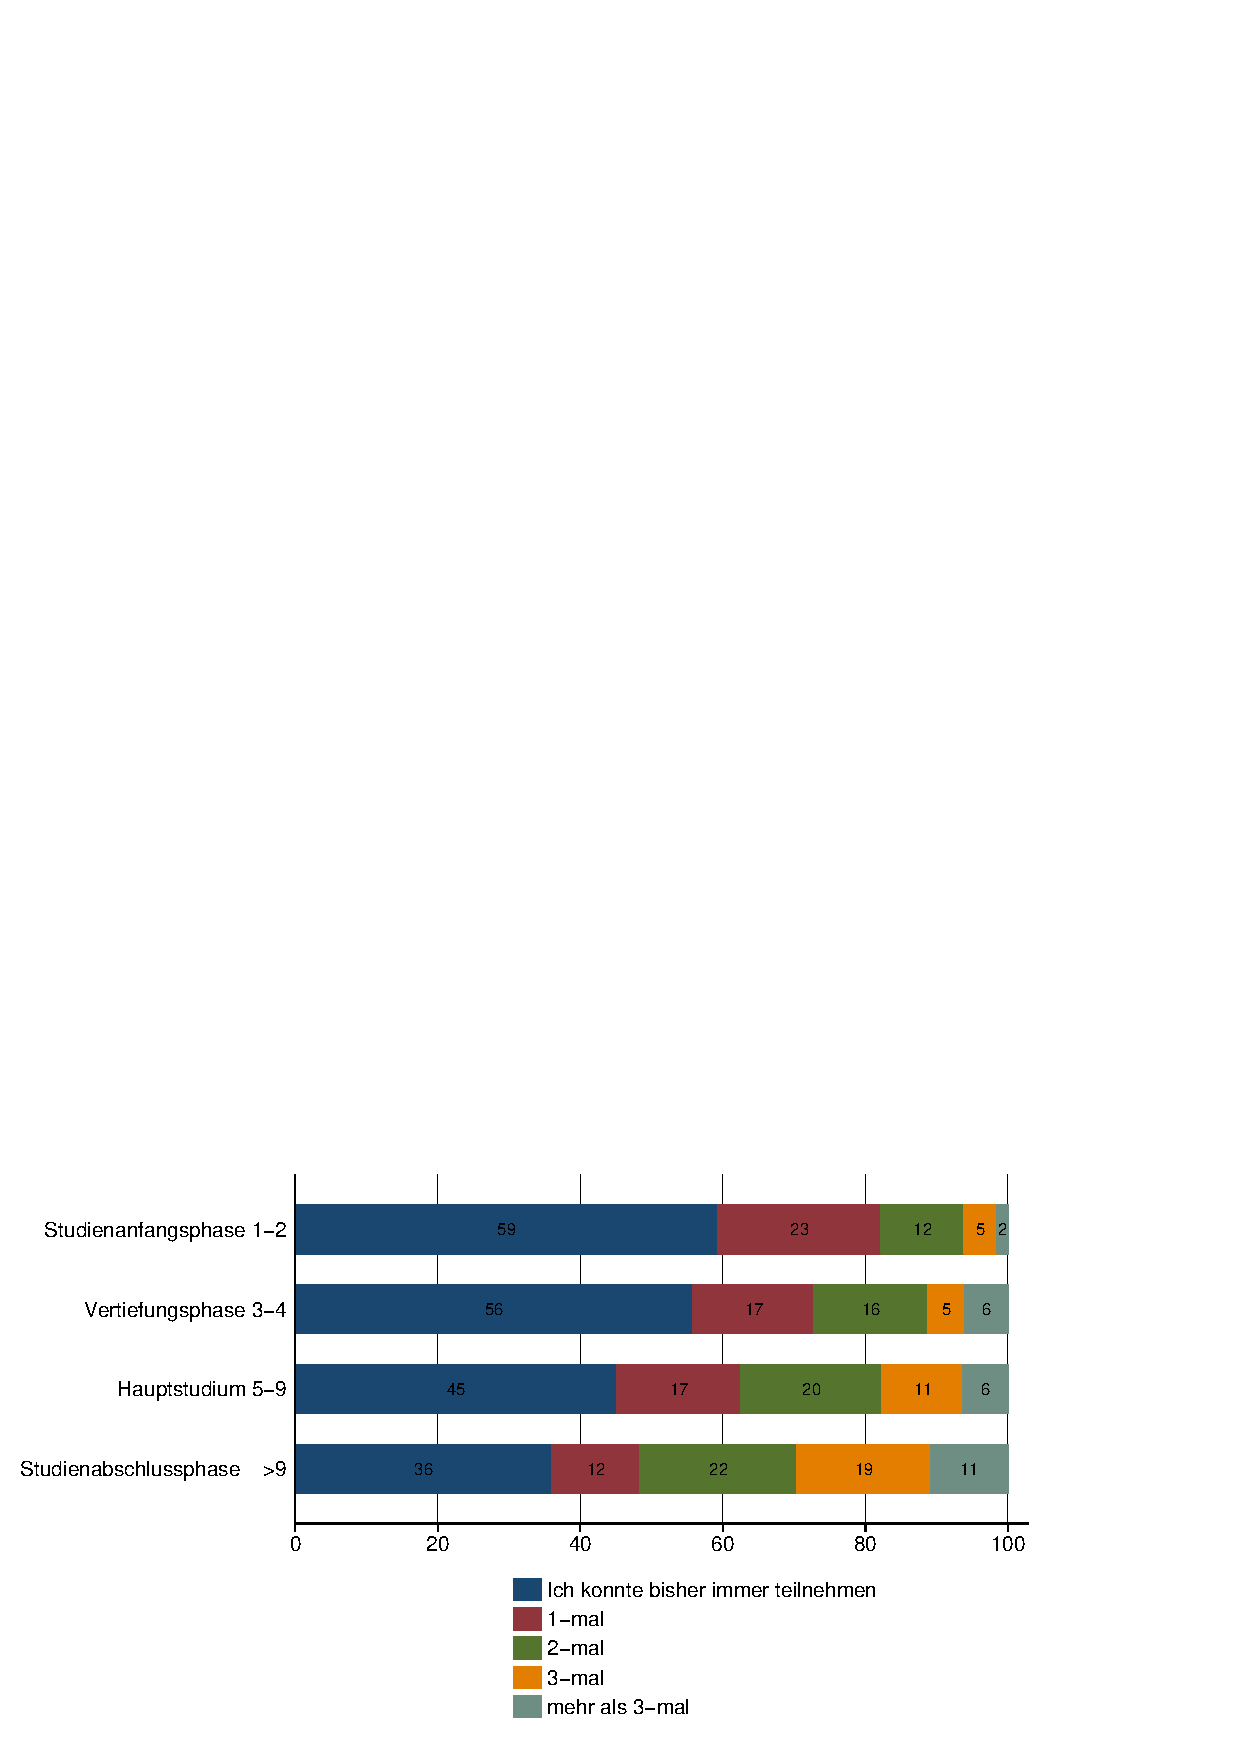
\includegraphics[width=0.5\textwidth]{image}
\end{verbatim} 
, the situation is more complicated. If you are using  \verb"\includegraphics" without the extension, pdfLaTeX when used with epstopdf or {\pack} looks for files that can be used in the following order:
\begin{verbatim}
Package grfext Info: Graphics extension search list:
(grfext)             [.png,.pdf,.jpg,.mps,.jpeg,.jbig2,.jb2,.PNG,.PDF,
.JPG,.JPEG,.JBIG2,.JB2,.eps]
\end{verbatim}
If - for whatever reason, a file \verb"image.png" exists, this one will be used, not the .eps or the converted pdf. However, you can use the option prepend the \enquote{Graphics extension search list} will look like this:
\begin{verbatim}
Package grfext Info: Graphics extension search list:
(grfext)             [.eps,.png,.pdf,.jpg,.mps,.jpeg,.jbig2,.jb2,.PNG,.PDF,
.JPG,.JPEG,.JBIG2,.JB2]
\end{verbatim}
This implies that image.eps is found first and used if a conversion to pdf is necessary. Complicated? Consider to use \verb"\includegraphics" \emph{with} the extension. This avoids confusion which file actually makes it into your document. See options prepend, prefersuffix, update, suffix below and try to figure out how many different scenarios there are. 



\section{Options}

{\pack} accepts several options.  Table \ref{optiontable} below gives an overview. The explanations are more or less taken from the documentation of  epspdf and epstopdf. 

%Put the following code in your main document. store the table in an extra-tex-file named LongTable.tex that might live in a subfolder Tables

\LTXtable{\textwidth}{optionstable.tex}


When there are several options in the first column, divided by |, this means that you should \emph{choose only one} of them. For example, it does not make sense have this in the preamble:
\begin{verbatim}
\usepackage[pdfversion=1.3,pdfversion=1.4]{epspdfconversion}
\end{verbatim}

\verb"\pdfminorversion": When you choose the options pdfversion=1.2 or pdfversion=1.3, you need to set \verb"\pdfminorversion" accordingly. The package checks if you have done that properly and shows a warning if not.


Changing the options somewhere in the middle of your .tex document is supported. Writing
\begin{verbatim}
\epspdfconversionsetup{target=prepress,bbox}
\end{verbatim}
changes the options of {\pack} to \verb"target=prepress,bbox". Other options than \verb"target=..." remain in effect.


\section{\textbackslash\texttt{epspdfconversioncmdline}}

Many of the options described above change the command that is used to call epspdf for the conversion from .eps to .pdf. %

Typing \verb"\epspdfconversioncmdline" somewhere in your source-.tex file will output the call that you have defined in your preamble. For example, this file has in the preamble

\begin{verbatim}
\usepackage[pdfversion=1.3,GRAY]{epspdfconversion}
\end{verbatim}

and the \verb"\epspdfconversioncmdline" then is:  \verb"epspdf --GRAY --version=1.3".

This means that you can use \verb"\renewcommand" to define you own \verb"\epspdfconversioncmdline". 

For example, to restore the behaviour of the epstopdf-package, you could write
%
\begin{verbatim}
\renewcommand{\epspdfconversioncmdline}%
{epstopdf }
\end{verbatim}
%
This allows you to use whatever tool you want for your eps->pdf conversion.


%\section{A test}
%
%What follows is the output of the \verb"\includegraphics"-command from page \pageref{bilderbefehle}.
%
%
%\begin{center}
%\includegraphics[width=0.5\textwidth]{image.eps}
%\end{center}

\section{Switching options temporarily}

It is possible to switch the options only temporarily using curly braces. Consider you have set the options \verb"GRAY" such that all your figures appear in grayscale. Now you want color for a single figure. This can be done like this:
%
\small
\begin{verbatim}
{% <= New group started
\epspdfconversionsetup{nogray,bbox=false}
\fbox{\includegraphics[width=4cm]{image2.eps}}
}% <= New group ended; grayscaling,bbox set to previous value.
\includegraphics[width=4cm]{image2.eps}
\end{verbatim}
\normalsize

The figure \verb"image2.eps" will be exceptionally in color, other figures in gray, according to the general rule for this document:

{% <= New group started
\epspdfconversionsetup{nogray,bbox=false}
\fbox{\includegraphics[width=4cm]{image2.eps}}
}% <= New group ended; grayscaling,bbox set to previous value.
\includegraphics[width=4cm]{image.eps}
 
\section{A note for users of latexmk}

(pdf)latexmk is a perl script for running LaTeX, BibTex, Makeindex etc the correct number of times. See \url{http://www.phys.psu.edu/~collins/software/latexmk/}. It can be configured to run pdflatex if an eps-image has been updated (since version V. 3.21i) -- hence updating an eps-file is considered to be an update of the document. In your local configuration file, you should have something like this: 

\small
\begin{verbatim}
# FOR USERS OF epstopdf v1.5 and later only:
add_cus_dep('eps', 'pdf', 0, 'cus_dep_require_primary_run');
\end{verbatim}
\normalsize

This makes latexmk to pay attention for .eps-files. If they are updated, pdflatexmk triggers a run of pdflatex (uses the subroutine \verb+cus_dep_require_primary_run+) and {\pack} can do the necessary conversion of the file.\footnote{If you enable the options pdftopdf and pstopdf, you should add the corresponding configuration.} 

Note that both epstopdf and latexmk are under active development. If you have difficulties to use latexmk together with  {\pack}, please let me know.

%\section{--help of epstopdf}
%
%The help of epspdf (version 0.5) reads:
%%
%\small
%\begin{verbatim}
%Daniels-MacBook:~ danielb$ epspdf --help
%Epspdf version 0.5
%Copyright (C) 2006, 2008, 2009, 2010 Siep Kroonenberg
%Convert between [e]ps and pdf formats
%Usage: epspdf.rb [options] infile [outfile]
%
%Default for outfile is file.pdf if infile is file.eps or file.ps
%Default for outfile is file.eps if infile is file.pdf
%
%    -g, --gray, --grey               Convert to grayscale;
%                                     success not guaranteed
%    -G, --GRAY, --GREY               Try harder to convert to grayscale
%    -p, --pagenumber=PAGENUMBER      Page to be converted or selected
%    -b, --bbox, --BoundingBox        Compute tight boundingbox
%    -n, --no-hires                   Don't use hires boundingbox
%    -r, --hires                      Use hires boundingbox
%    -T, --target=TARGET              Target use of pdf; one of
%                                     default, printer, prepress, screen, ebook
%    -N, --pdfversion=PDFVERSION      Pdf version to be generated
%    -V, --version=PDFVERSION         Deprecated; use `-N' or `--pdfversion'.
%    -I                               Ignore pdftops even if available
%                                     (default: use if available)
%    -U                               Use pdftops if available
%                                     (overrides previous -I setting)
%    -C, --custom=CUSTOMOPTIONS       Custom options for conversion to pdf,
%                                     view Use.htm and ps2pdf.htm from
%                                     the Ghostscript documentation set
%    -P, --psoptions=PSOPTIONS        Options for pdftops; default -level3,
%                                     don't include -eps or page number options;
%                                     these will be generated by the program
%    -i, --info                       Info: display detected filetype
%    -s                               Save (some) settings
%    -d                               Debug: don't remove temp files
%        --gui[=ACTION]               Do not use; reserved for GUI
%
%    -v                               Prints version info
%    -h, --help                       Show this message
%\end{verbatim}
%\normalsize



%\vfill

\small 
\section{Version-history, ToDo's}

\begin{description}
  \item[Possible ToDo's] add support for tif and others in pdflatex via convert / add support for pdf-inclusion in latex (not pdf-latex) / add support for more file-types (tif, jpeg,...) in latex (not pdf-latex) / add support for sam2p.
  
  Please report errors, missing features and other suggestions.
 \item[v.0.61, 2010-06-1:]
 \begin{itemize}
  \item new options pdftopdf and pstopdf. Uses epspdf to do pdf-to-pdf and ps-to-pdf conversions. Allows grayscaling, calculation of 
bounding boxes etc for pdf's that already exist an for .ps-files. Disabled by default.
  \item bugfix for the outdir-option (converted files in subdirectories are again saved in those subdirectories)
      (Thanks to Stefan Pofahl for the feedback.)
  \item small improvement of the documentation (on the windows epspdf.bat file, on epstopdf's option 'outdir')
  \item now uses epstopdf's \verb"\epstopdfDeclareGraphicsRule"
\end{itemize}
  \item[v.0.6, 2010-04-30:] small improvements and documentation updates
  \begin{itemize}
  \item  pdfversion now uses epspdf's --pdfversion. --version in epspdf is to print the version number of epspdf (currently, epspdf is at 0.5)
  \item new author email
  \item documentation updates
\end{itemize}
  \item[v.0.5, 2009-09-02:] this update makes use of changes in the epstopdf-package v2.2\begin{itemize}
  \item new options 
        update,verbose,prefersuffix,suffix,outdir
        (they are really epstopdf options, but can be set 
        as options for this package)
  \item default is that converted files have a suffix
  \item info in logfile about the setup that is used for epstopdf
  \item new options hires, no-hires
\end{itemize} 
  \item[v.0.4, 2007-11-24:] the epstopdf-package is now loaded with options [update,prepend] (works only when epstopdf version 1.5 is used) An update of epstopd.sty (part of the oberdiek-bundle) is recommended. Added options nogrey,nogray
  \item[v.0.3, 2007-10-02:] \begin{itemize}
  \item check whether \verb"\pdfminorversion" has been set in accordance with option pdfversion=...
  \item Use the kvoptions-package for the implemention of options. It uses key value syntax that can be used both as package options and a separate setup macro.
  \item Almost all options of epstopdf are now available as an option of this package.
  \item The command \verb"\epspdfconversionsetup" is new and allows a change of the options for this package anywhere in your document.
  \item The command \verb"\epspdfconversioncmdline" has been renamed to\\ \verb"\epspdfconversioncmdline".
  \item the documentation has been updated
\end{itemize}   
  \item[v.0.2, 2007-09-21:] the package is now simply based on epstopdf. It essentially defines \\ \verb"\@namedef{Gin@rule@.eps}#1{{pdf}{.pdf}{`\epspdfconversioncmdline #1}}" differently than epstopdf. The code has been cleaned up. Improvements of documentation and additional warning about pdfminorversion....
  \item[v.0.1, 2007-09-21:] first try
\end{description}

\end{document}
 